% Intended LaTeX compiler: pdflatex
\documentclass[11pt]{article}
\usepackage[utf8]{inputenc}
\usepackage[T1]{fontenc}
\usepackage{graphicx}
\usepackage{longtable}
\usepackage{wrapfig}
\usepackage{rotating}
\usepackage[normalem]{ulem}
\usepackage{amsmath}
\usepackage{amssymb}
\usepackage{capt-of}
\usepackage{hyperref}
\author{Construção de compiladores I}
\date{}
\title{Apresentação da disciplina}
\hypersetup{
 pdfauthor={Construção de compiladores I},
 pdftitle={Apresentação da disciplina},
 pdfkeywords={},
 pdfsubject={},
 pdfcreator={Emacs 28.2 (Org mode 9.7)}, 
 pdflang={English}}
\begin{document}

\maketitle
\section*{Objetivos}
\label{sec:orge7d13e4}

\subsection*{Objetivos}
\label{sec:orgffc5eee}

\begin{itemize}
\item Apresentar a importância da construção de compiladores na formação de um cientista da computação.
\item Apresentar a ementa, critérios de avaliação e bibliografia da disciplina.
\end{itemize}
\subsection*{Objetivos}
\label{sec:orgd231040}

\begin{itemize}
\item Apresentar a visão geral de um compilador.
\end{itemize}
\section*{Motivação}
\label{sec:orgc37fe1e}

\subsection*{Compiladores}
\label{sec:org2c51b98}

\begin{itemize}
\item Peça central da ciência da computação.
\begin{itemize}
\item Tarefa: traduzir programas de ``alto nível'' em código de máquina
\item Tecnologia responsável pelo grande avanço da computação!
\end{itemize}
\end{itemize}
\subsection*{Compiladores}
\label{sec:orgff16b52}

\begin{itemize}
\item Desenvolver um compilador permite consolidar conhecimentos de:
\begin{itemize}
\item Estruturas de dados e algoritmos (árvores, grafos, etc\ldots{})
\end{itemize}
\end{itemize}
\subsection*{Compiladores}
\label{sec:org2899906}

\begin{itemize}
\item Desenvolver um compilador permite consolidar conhecimentos de:
\begin{itemize}
\item Teoria da computação (autômatos e gramáticas)
\end{itemize}
\end{itemize}
\subsection*{Compiladores}
\label{sec:org31b4d5e}

\begin{itemize}
\item Desenvolver um compilador permite consolidar conhecimentos de:
\begin{itemize}
\item Engenharia de software (testes e arquitetura de software)
\end{itemize}
\end{itemize}
\subsection*{Compiladores}
\label{sec:org2ce5d54}

\begin{itemize}
\item Desenvolver um compilador permite consolidar conhecimentos de:
\begin{itemize}
\item Arquitetura de computadores (conhecer detalhes do alvo de compilação)
\end{itemize}
\end{itemize}
\subsection*{Compiladores}
\label{sec:org7b157d7}

\begin{itemize}
\item Possivelmente, o primeiro artefato de software complexo produzido por estudantes de graduação.
\end{itemize}
\subsection*{Compiladores}
\label{sec:org7181bb5}

\begin{itemize}
\item Compiladores aparecem em toda parte!
\begin{itemize}
\item Navegadores web (JavaScript e WebASM)
\item Monitoramento do Kernel Linux (eBPF)
\item Várias aplicações possuem linguagens para customização.
\end{itemize}
\end{itemize}
\subsection*{Compiladores}
\label{sec:orgb21c22c}

\begin{itemize}
\item Projeto de compiladores envolve problemas difíceis:
\begin{itemize}
\item Executam várias tarefas e devem ser eficientes.
\end{itemize}
\end{itemize}
\subsection*{Compiladores}
\label{sec:org83aee84}

\begin{itemize}
\item Projeto de compiladores envolve problemas difíceis:
\begin{itemize}
\item Responsáveis por bom uso de uma linguagem.
\end{itemize}
\end{itemize}
\subsection*{Compiladores}
\label{sec:org22cc0a2}

\begin{itemize}
\item Projeto de compiladores envolve problemas difíceis:
\begin{itemize}
\item Devem ocultar detalhes de arquiteturas de desenvolvedores.
\end{itemize}
\end{itemize}
\subsection*{Compiladores}
\label{sec:org8f7378a}

\begin{itemize}
\item Provavelmente, uma das áreas mais consolidadas da ciência da computação!
\end{itemize}
\subsection*{Compiladores}
\label{sec:org3e72f21}

\begin{itemize}
\item Vários pesquisadores da área foram agraciados com o Turing Award!
\begin{itemize}
\item John Backus, Barbara Liskov, Niklaus Wirth, Edsger Djikstra e C.A. Hoare.
\end{itemize}
\end{itemize}
\subsection*{Compiladores}
\label{sec:org85233e7}

\begin{itemize}
\item Mas porque criar compiladores?
\begin{itemize}
\item Criar novas linguagens para facilitar tarefas de desenvolvimento.
\item Exemplos: Lua, Elixir, Elm, Rust, Scala e outras linguagens
\end{itemize}
\end{itemize}
\subsection*{Compiladores}
\label{sec:org9d266e0}

\begin{itemize}
\item Conteúdo aplica-se somente a criar novas linguagens?
\begin{itemize}
\item Não! Diversas ferramentas úteis utilizam conceitos de compiladores.
\end{itemize}
\end{itemize}
\section*{Ementa}
\label{sec:org24259c3}

\subsection*{Ementa}
\label{sec:org5538aed}

\begin{itemize}
\item Revisão de programação funcional em Haskell
\item Introdução ao processo de compilação e interpretação
\end{itemize}
\subsection*{Ementa}
\label{sec:org1540b9b}

\begin{itemize}
\item Análise léxica

\item Análise sintática

\item Análise semântica e geração de código intermediário.
\end{itemize}
\section*{Bibliografia}
\label{sec:orgaef4056}

\subsection*{Bibliografia}
\label{sec:org6487789}

\begin{itemize}
\item Construindo Compiladores. Cooper, Keith D. ; Torcson, Linda

\item Compiladores: Princípios, técnicas e ferramentas. Aho, Alfred; Lam, Monica; Sethi, Ravi; Ullman, Jeffrey.

\item Modern compiler implementation in ML. Appel, Andrew.
\end{itemize}
\section*{Materiais de apoio}
\label{sec:org36c033a}

\subsection*{Materiais de apoio}
\label{sec:org6881e7e}

\begin{itemize}
\item Slides e código de exemplo serão disponibilizados no seguinte repositório online.
\end{itemize}
\section*{Critérios de Avaliação}
\label{sec:org4821a03}

\subsection*{Critérios de Avaliação}
\label{sec:orgb6e7872}

\begin{itemize}
\item Uma avaliação no valor de 4,0 pontos.

\item Trabalhos práticos e exercícios de programação no valor 6,0 pontos.
\end{itemize}
\subsection*{Critérios de Avaliação}
\label{sec:org6a91f14}

\begin{itemize}
\item Avaliação versa sobre o conteúdo teórico da disciplina:
\begin{itemize}
\item Funcionamento de algoritmos
\item Semântica de linguagens de programação
\item Sistemas de tipos
\end{itemize}
\end{itemize}
\subsection*{Critérios de Avaliação}
\label{sec:orgbfb13c8}

\begin{itemize}
\item Trabalhos práticos sobre o conteúdo
\begin{itemize}
\item Extensão de protótipos de compiladores apresentados na disciplina.
\item Desenvolvimento de um projeto de ferramenta que utiliza técnicas de compilação.
\end{itemize}
\end{itemize}
\subsection*{Critérios de Avaliação}
\label{sec:org0de5b08}

\begin{itemize}
\item Entregas de trabalhos
\begin{itemize}
\item Entrega 1: 25/10/2023
\item Entrega 2: 18/11/2023
\item Entrega 3: 29/01/2024
\end{itemize}
\end{itemize}
\subsection*{Critérios de Avaliação}
\label{sec:org1c77d22}

\begin{itemize}
\item Exercícios de programação
\begin{itemize}
\item Datas de entrega a serem determinadas na plataforma Moodle.
\end{itemize}
\end{itemize}
\subsection*{Critérios de Avaliação}
\label{sec:org7a72d64}

\begin{itemize}
\item Data avaliação: 05/02/2024
\end{itemize}
\subsection*{Exame especial}
\label{sec:org2c8219d}

\begin{itemize}
\item Mínimo de 75\% de frequência e nota inferior a 6,0.

\item Exame especial parcial para alunos que perderam uma avaliação.
\begin{itemize}
\item Envolverá tarefas de codificação e atividades teóricas (em papel).
\end{itemize}

\item Detalhes: Resolução CEPE 2880 de 05/2006
\end{itemize}
\subsection*{Exame especial}
\label{sec:orgb54b02d}

\begin{itemize}
\item Data do exame especial: 19/02/2024
\end{itemize}
\section*{Software}
\label{sec:orgb186b2e}

\subsection*{Software}
\label{sec:org6d23779}

\begin{itemize}
\item Trabalhos e códigos de exemplo serão desenvolvidos utilizando Haskell.

\item Utilizaremos diversas bibliotecas da linguagem Haskell.
\end{itemize}
\subsection*{Software}
\label{sec:orgdeef940}

\begin{itemize}
\item Infraestrutura para desenvolvimento de trabalhos está configurada utilizando o gerenciador de pacotes \href{https://nixos.org/}{Nix}.

\item Gerenciador de pacotes Nix pode ser instalado em Windows, Linux e MacOS.
\end{itemize}
\subsection*{Software}
\label{sec:orgae3905a}

\begin{itemize}
\item Utilizando o Nix, você conseguirá um ambiente consistente para desenvolvimento de trabalhos e exercícios.
\begin{itemize}
\item Versão correta de compilador, bibliotecas e ferramentas auxiliares.
\end{itemize}
\end{itemize}
\subsection*{Software}
\label{sec:org4c8ce37}

\begin{itemize}
\item Recomanda-se \textbf{\textbf{FORTEMENTE}} o uso do Nix para garantir o mesmo ambiente de execução para trabalhos.

\item Código que não executar no ambiente, não será considerado para correção.
\end{itemize}
\section*{Outras informações}
\label{sec:org8819d68}

\subsection*{Informações}
\label{sec:orgcdc6e48}

\begin{itemize}
\item Toda informação da disciplina será disponibilizada na plataforma Moodle.

\item Email: rodrigo.ribeiro@ufop.edu.br
\end{itemize}
\subsection*{Atendimento}
\label{sec:org5c0b379}

\begin{itemize}
\item Segunda-feira: 08:00 - 10:00h e 15:30-17:30h.
\item Quarta-feira: 08:00 - 10:00h.
\end{itemize}
\subsection*{Finalizando}
\label{sec:orga30a90e}

\begin{itemize}
\item Tenhamos todos um excelente semestre de trabalho!
\end{itemize}
\section*{Motivação}
\label{sec:org8189118}

\subsection*{Compiladores}
\label{sec:orgeb6e0cc}

\begin{itemize}
\item Peça central da ciência da computação.
\begin{itemize}
\item Tarefa: traduzir programas de ``alto nível'' em código de máquina
\item Tecnologia responsável pelo grande avanço da computação!
\end{itemize}
\end{itemize}
\subsection*{Compiladores}
\label{sec:org549bf61}

\begin{itemize}
\item Nosso objetivo, responder a pergunta:
\begin{itemize}
\item Como um compilador funciona?
\end{itemize}
\end{itemize}

\begin{center}

\includegraphics[width=.9\linewidth]{./imgs/image1.png}
\end{center}
\subsection*{Compiladores}
\label{sec:org9ba53c8}

\begin{itemize}
\item Um compilador deve:
\begin{itemize}
\item Detectar todos os erros e reportá-los
\item Deve preservar a semântica do programa de entrada.
\item Realizar interface do programa com o SO.
\end{itemize}
\end{itemize}
\subsection*{Interpretadores}
\label{sec:orged7a829}

\begin{itemize}
\item Estrutura geral de um interpretador
\end{itemize}

\begin{center}
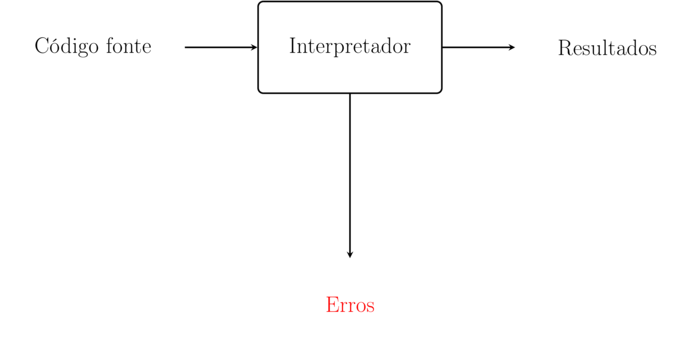
\includegraphics[width=.9\linewidth]{./imgs/image2.png}
\end{center}
\subsection*{Compiladores}
\label{sec:orgfd5ab1e}

\begin{itemize}
\item Estrutura de alto nível
\end{itemize}

\begin{center}
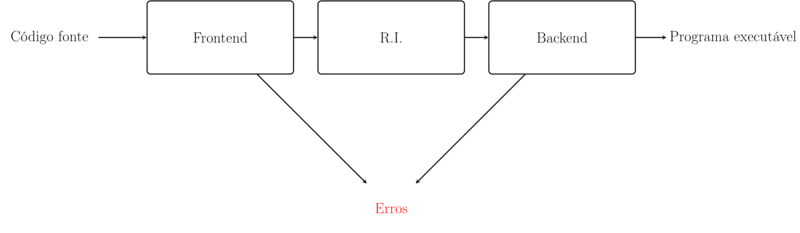
\includegraphics[width=.9\linewidth]{./imgs/image3.png}
\end{center}
\section*{Frontend}
\label{sec:orgd1a323d}

\subsection*{Frontend}
\label{sec:orgb1ac79f}

\begin{itemize}
\item Responsável pela análise do código fonte.
\begin{itemize}
\item Deve detectar e reportar todos os erros antes da geração de código.
\item Deve produzir uma representação intermediária do código fonte.
\end{itemize}
\end{itemize}
\subsection*{Frontend}
\label{sec:org7259492}

\begin{itemize}
\item Estrutura do frontend
\end{itemize}

\begin{center}
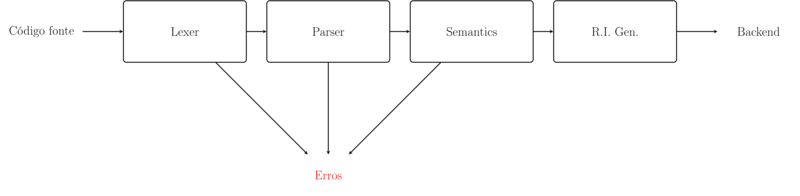
\includegraphics[width=.9\linewidth]{./imgs/image4.png}
\end{center}
\section*{Estrutura de um frontend}
\label{sec:org16b7564}

\subsection*{Analisador léxico}
\label{sec:org90a4282}

\begin{itemize}
\item Componente responsável por identificar elementos do ``alfabeto'' da linguagem
\begin{itemize}
\item Normalmente chamados de ``tokens''.
\end{itemize}

\item Responsável por eliminar espaços em branco e comentários da entrada.
\end{itemize}
\subsection*{Analisador léxico}
\label{sec:org2ddf42c}

\begin{itemize}
\item Capaz de identificar erros simples de digitação de palavras chave.
\begin{itemize}
\item Ex: ``wihle'' ao invés de ``while''.
\end{itemize}

\item Resultado: Lista de tokens.

\item Formalismo: autômatos finitos e linguagens regulares.
\end{itemize}
\subsection*{Analisador sintático}
\label{sec:orgc2ebca0}

\begin{itemize}
\item Componente responsável por identificar estrutura gramatical.

\item Capaz de identificar uma grande quantidade de erros.
\begin{itemize}
\item Ex. Esquecer um ``;'' no fim de um comando.
\item Ex. Não usar parêntesis balanceados.
\end{itemize}
\end{itemize}
\subsection*{Analisador sintático}
\label{sec:org433bfd3}

\begin{itemize}
\item Resultado: Árvore de sintaxe abstrata (AST).

\item Formalismo: Gramáticas livres de contexto e autômatos de pilha.
\end{itemize}
\subsection*{Analisador semântico}
\label{sec:org0a96bab}

\begin{itemize}
\item Responsável por validar regras semânticas da linguagem
\begin{itemize}
\item Todo uso deve possuir declaração correspondente.
\item Regras de tipo.
\end{itemize}

\item Resultado: AST com anotações de tipos.
\end{itemize}
\subsection*{Gerador de IR}
\label{sec:orgcfa6002}

\begin{itemize}
\item Responsável por converter a AST em uma representação um pouco
mais próxima do código final.

\item Em algumas situações, a própria AST é uma possível IR.
\end{itemize}
\subsection*{Gerador de IR}
\label{sec:org0c27e3b}

\begin{itemize}
\item Neste curso, vamos usar a LLVM.
\begin{itemize}
\item Framework para construção de backends usando a forma SSA.
\end{itemize}

\item Também veremos como gerar código para uma máquina de pilha.
\begin{itemize}
\item Simplificação da JVM / EVM.
\end{itemize}
\end{itemize}
\section*{Conclusão}
\label{sec:org81e22ce}

\subsection*{Conclusão}
\label{sec:org73edea8}

\begin{itemize}
\item Próximas aulas: revisão de Haskell
\begin{itemize}
\item Compilador de um subconjunto de markdown.
\end{itemize}
\end{itemize}
\end{document}
